% 第四章 基于DispNetC的立体匹配

\chapter{基于DispNetC的立体匹配}
% ref: FlowNet paper ch2, Convolutional Networks part.
2012年Krizhevsky等人的工作\cite{krizhevsky2012imagenet}展示了卷积神经网络在大规模图像分类中的良好效果,带动了应用CNN到各种计算机视觉任务中的研究工作。深度卷积神经网络较传统神经网络而言,能够学习到更为复杂的非线性关系,因此能够更好地从大量数据中提取规律。同时其通过卷积操作获得的特征也比人工设计的特征更为有效。

过去几年涌现出了大量使用CNN进行立体匹配的研究成果。KITTI\cite{Menze_2015_CVPR} Stereo Evaluation排行榜的前列已被基于卷积神经网络的算法占领,此类算法在匹配精度和运行时间方面较传统方法都展现出了很明显的优势。Fisher等人\cite{fischer2014descriptor}从通过有监督/无监督训练得到的CNN中提取特征表达,并基于欧氏距离对这些特征进行匹配。Zbontar和LeCun\cite{zbontar2016stereo}训练了一个连体(Siamese)架构的CNN,用来预测图像块之间的相似度。这类基于图像块(patch)的算法的缺点是计算量较大,无法利用全局信息,在计算完匹配代价后仍然需要进行后处理操作,因此并不能显著降低算法的运行时间。

DispNet\cite{mayer2016large}是一种网络结构较为简单、端到端(end-to-end)的立体匹配网络。该网络的运行速度很快,适合应用于无人机等对实时性有较高要求的场景。本章介绍DispNet的网络结构、训练过程并给出使用其进行立体匹配的结果。

%------------------------------------------------------------------------------------
\section{DispNet网络结构}
% ref: FlowNet paper ch3; DispNet paper ch5.
DispNet是一种端到端的立体匹配卷积神经网络模型。所谓“端到端”是指输入需要匹配的左右图,即可预测得到匹配结果,无需其他后处理操作。其借鉴了用于预测光流的FlowNet\cite{dosovitskiy2015flownet}的结构并将其应用于立体匹配领域。

在卷积神经网络中,池化对于降低训练网络的训练量是必要的,而且能够使得网络具备聚合输入图像中更大范围信息的能力。但是池化会导致分辨率下降,为了获得稠密的与输入图像具有相同分辨率的预测结果,我们需要对池化后得到的粗糙结果进行细化。因此DispNet网络的结构呈沙漏形(如图\ref{fig:4_1_dispnet_shape}),包含一个收缩部分和一个扩张部分,整个网络作为一个整体,使用反向传播算法来训练。

\begin{figure}[!htbp]
	\centering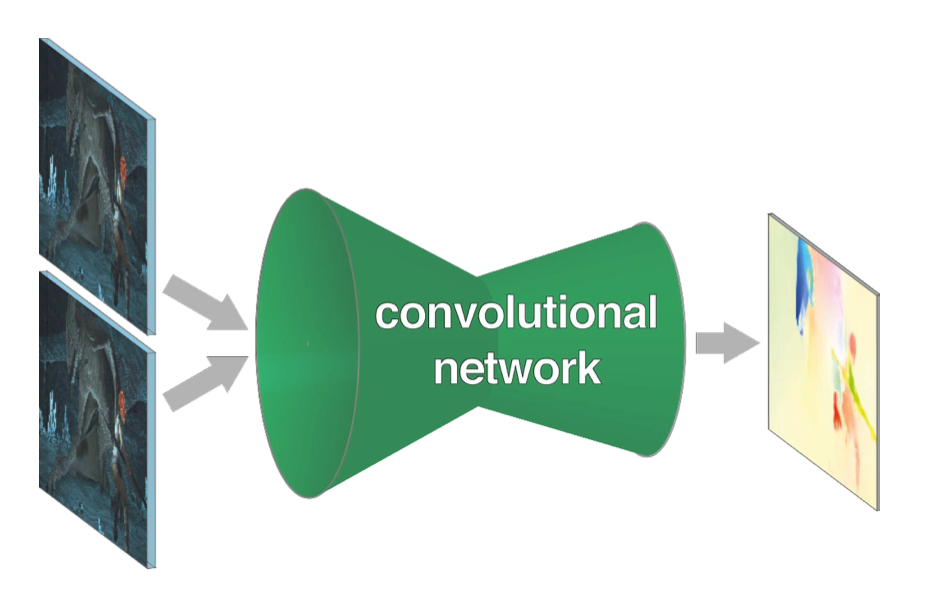
\includegraphics[width=3.5in]{figures/4_1_dispnet_shape.png}
	\caption{沙漏型的网络结构\cite{dosovitskiy2015flownet}}\label{fig:4_1_dispnet_shape}
\end{figure}

\subsubsection{收缩部分}
DispNet的收缩部分包括10个卷积层,其中前两个卷积层的卷积核尺寸分别为$7\times 7$和$5\times 5$,其余卷积层的卷积核尺寸为$3\times 3$。10个卷积层中有6个取步长为2,其余为1,故一共进行了64倍的下采样。

网络的输入为一对图片,最简单的处理方式是将两张图片直接堆叠在一起输入网络,让网络自己学习如何处理成对的图像来获取所需的深度信息。每张图片有RGB三个通道,故网络输入的厚度为6。这种只包含卷积层的网络架构是DispNet的基础架构,如图\ref{fig:4_1_DispNet}所示。图中标注的数字为“分辨率@通道数(特征图层数)”。

\begin{figure}[!htbp]
	\centering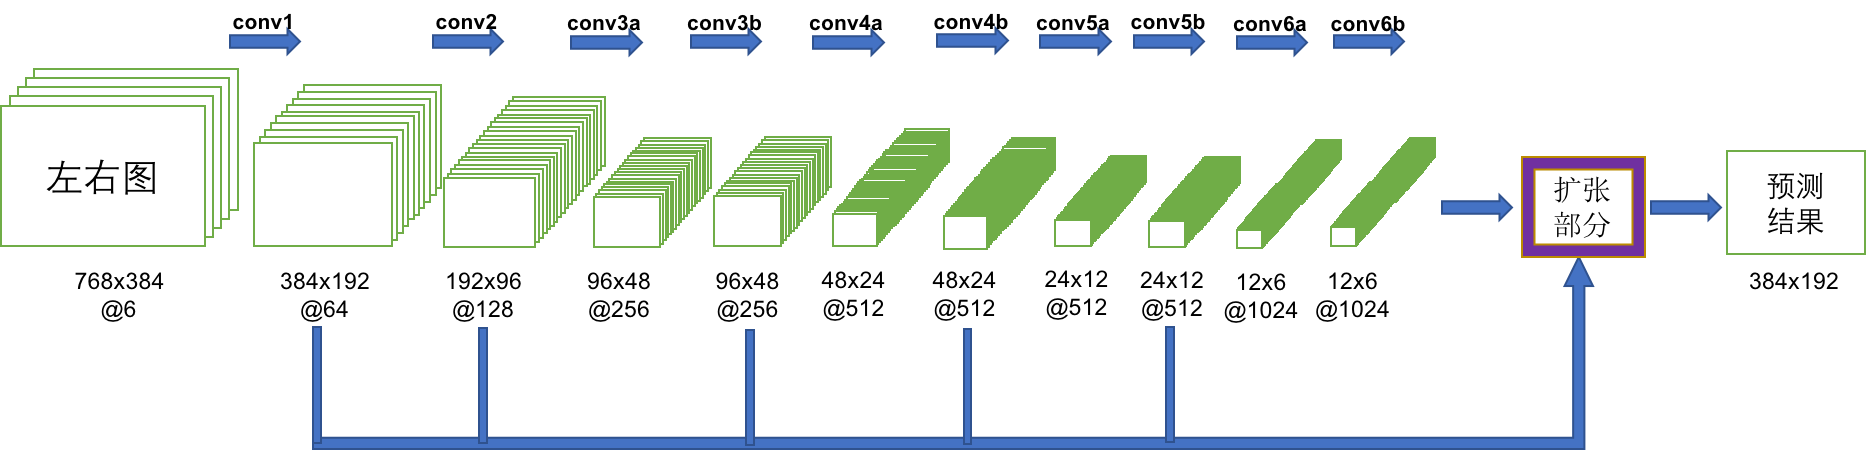
\includegraphics[width=6in]{figures/4_1_dispnet_architecture}
	\caption{DispNet网络基础架构}\label{fig:4_1_DispNet}
\end{figure}

另一种处理方式是建立两个相互独立但相同的结构来分别处理输入的左右图,之后通过一定方式将它们组合起来,如图\ref{fig:4_1_DispNetC}所示。网络首先分别从两张图片生成一些有价值的特征表达,然后在更高级别将它们联系起来。这种结构有些类似于传统的匹配模式:首先从两张图片的小块区域中提取特征,然后比较获得的特征向量。

\begin{figure}[!htbp]
	\centering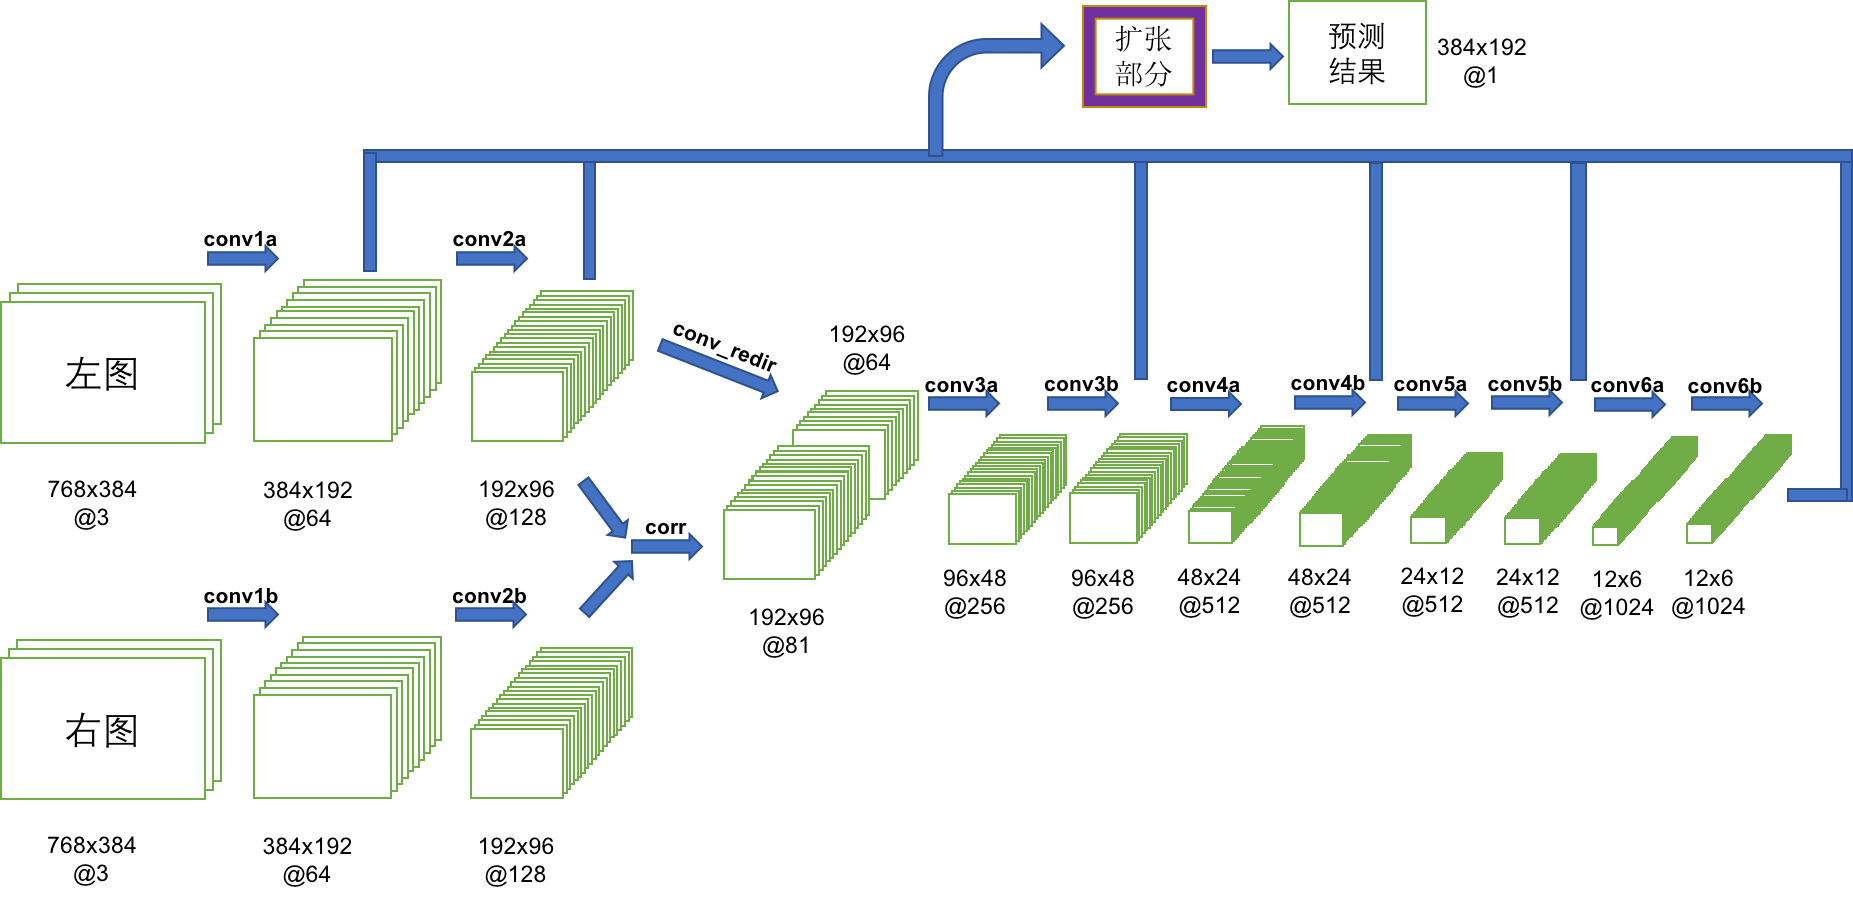
\includegraphics[width=6in]{figures/4_1_dispnetc_architecture}
	\caption{DispNetC网络架构}\label{fig:4_1_DispNetC}
\end{figure}

FlowNet中引入了一个“相关层(correlation layer)”来进行两个特征图之间的比较。假设有两个多通道的特征图
$f_1, f_2: \mathbb{R} \rightarrow \mathbb{R}^c$,$w$,$h$和$c$ 
分别是他们的宽度、高度和通道数。相关层可以让网络比较$f_1$和$f_2$中的每个小块(patch)。为了说明相关层的计算方式,下面只考虑某两个小块之间的比较。取边长为$K=2k+1$的方形小块,第一张特征图中以$x_1$为中心的小块与第二张特征图中以$x_2$为中心的小块的相关量定义为:
\begin{equation}\label{eq:4_1_correlation}  % 前面不要留空行,否则行间距大。
c(\mathbf{x}_1, \mathbf{x}_2) = \sum_{\mathbf{o} \in [-k, k] \times [-k, k]} { \langle \mathbf{f}_1(\mathbf{x}_1 + \mathbf{o}), \mathbf{f}_2(\mathbf{x}_2 + \mathbf{o}) \rangle }
\end{equation}

注意到方程\ref{eq:4_1_correlation}相当于神经网络中步长为1的卷积操作,区别在于这里是用数据与数据进行卷积,而不是使用卷积核,因此并没有可训练的权重参数。

计算$c(\mathbf{x}_1, \mathbf{x}_2)$需要进行$c\cdot K^2$次乘法。而遍历两图中所有的组合方式需要进行$w^2  \cdot h^2$次相关计算,如此大的计算量将无法实现高效的训练和预测。因此出于计算量的考虑,需要限制两图中patch的最大相对位移。设最大位移为$d$,则对于每个$\mathbf{x}_1$,$\mathbf{x}_2$被限制在$\mathbf{x}_1$附近$D=2d+1$的范围内,减小了两图中patch的组合数。另外,FlowNet在相关计算中还加入了步长$s_1, s_2$来进一步减小比较的数量。

由于立体匹配使用的图片是行对齐的,并没有必要进行二维的相关计算,因此简化为水平方向的一维相关计算。取最大相对位移$d$为40个像素,由于在进行相关计算之前图像已经经过了2个步长为2的卷积层,故这里40个像素对应输入图像的160个像素,已经覆盖了足够大的视差范围。相比FlowNet中的二维相关计算,采用一维相关计算大大减小了计算量,而且较FlowNet覆盖了更大的相对位移范围,同时因为不需使用步长,获得了更精细的采样。实际操作中,每个patch取为1个像素。因为加入了相关层,我们称这种网络结构为DispNetC。

%------------------------------------------------------------------------------------
\subsubsection{扩张部分}
扩张部分的主要结构是上卷积层(upconvolutional layer),由去池化(unpooling,与池化相对)和卷积组成。这种网络层已被多次使用过\cite{zeiler2011adaptive, zeiler2014visualizing, goodfellow2014generative}。为了获得精细的预测结果,我们对特征图应用上卷积,并将其和收缩部分中对应的特征图、以及上一层的较粗糙的预测结果拼接起来。这样既保留了从更粗糙的特征图传递过来的高级信息,也保留了更低网络层的特征图提供的精细局部信息。每一次上卷积使预测结果的分辨率增加一倍,一共重复4次上卷积,最终得到的预测结果的分辨率是输入图像的四分之一,宽度和高度都是原图的一半。对网络输出的结果使用插值方法即可获得与输入图像相同的分辨率。根据\cite{dosovitskiy2015flownet}的实验,继续增加上卷积层来细化预测结果相比使用双线性插值方法并不能显著提高预测精度,但由于视差必须取整数,我们使用最近邻插值来得到输入分辨率的结果。扩张部分的结构如图\ref{fig:4_1_DispNet_expanding_part}所示。

\begin{figure}[!htbp]
	\centering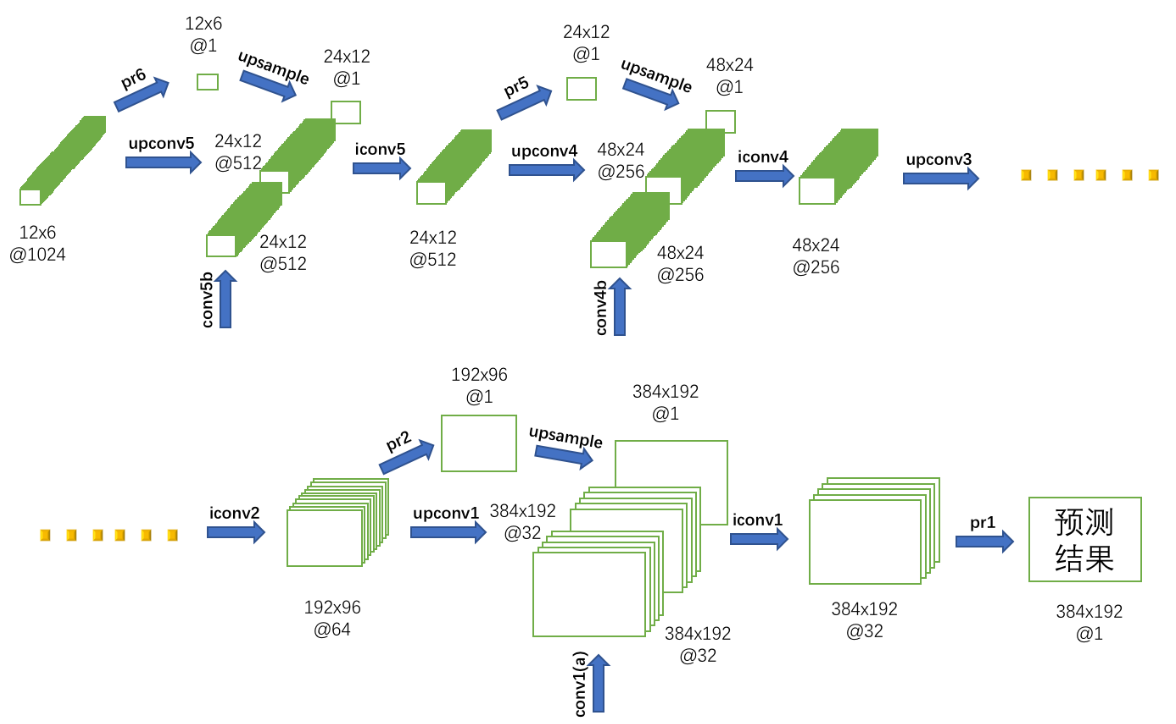
\includegraphics[width=6in]{figures/4_1_dispnet_expanding_part.png}
	\caption{DispNetC扩张部分结构}\label{fig:4_1_DispNet_expanding_part}
\end{figure}

DispNet网络结构的详细参数见表\ref{tab:4_1_DispNet_architecture}。收缩部分包括conv1到conv6b。扩张部分中,上卷积层(upconvN)、卷积层(iconvN,  prN)和代价层(loss)交替出现。最终模型预测的视差图为pr1层的输出。
DispNetC与基础架构的区别存在于前三层。只需要将基础架构的前两层(conv1, conv2)平均拆分为权值共享的两部分,conv1a/b层的输入通道数减小为3。conv2a/b层经过相关层(corr)后的输出通道数为$2d+1=81$,和con2a通过卷积重定向层(conv\_redir)后的结果拼接在一起,再通过conv3a将输出通道数与基础架构中conv3a的输出进行统一,其余部分与基础架构完全一致。
% leaky relu要不要介绍???
网络收缩部分每个卷积层使用的激活函数为Leaky ReLU,扩张部分不使用激活函数。

\begin{table}[htbp] % 这两个表格是不是应该放到附录里去。算了。
	\centering
	\caption{DispNet网络结构详细参数}
	\label{tab:4_1_DispNet_architecture}
	\begin{scriptsize}   % tiny, scriptsize, footnotesize, small.
		\begin{tabular}{|l|c c c|c c|c|}\hline
			网络层 & 卷积核 & 步长 & 输入/输出通道数 & 输入分辨率 & 输出分辨率 & 该层输入 \\\hline
			%---------------------------------------------------------
			conv1    & 7x7 & 2 & 6/64                & 768x384 & 384x192 & 左右图像 \\
			conv2    & 5x5 & 2 & 64/128           & 384x192  & 192x96    & conv1 \\
			conv3a & 5x5 & 2 & 128/256         & 192x96     & 96x48      & conv2 \\
			conv3b & 3x3 & 1 & 256/256        & 96x48       & 96x48      & conv3a\\
			conv4a & 3x3 & 2 & 256/512        & 96x48        & 48x24      & conv3b \\
			conv4b & 3x3 & 1 & 512/512         & 48x24        & 48x24       & conv4a \\
			conv5a & 3x3 & 2 & 512/512         & 48x24        & 24x12        & conv4b \\
			conv5b & 3x3 & 1 & 512/512         & 24x12          & 24x12       & conv5a \\
			conv6a & 3x3 & 2 & 512/1024     & 24x12          & 12x6          & conv5b \\
			conv6b & 3x3 & 1 & 1024/1024  & 12x6             & 12x6          & conv6a \\\hline
			%---------------------------------------------------------
			pr6+loss6 & 3x3 & 1 & 1024/1 & 12x6 & 12x6 & conv6b \\\hline
			%---------------------------------------------------------
			upconv5    & 4x4 & 2 & 1024/512  & 12x6        & 24x12    & conv6b \\
			iconv5        & 3x3 & 1 & 1025/512  & 24x12      & 24x12    & upconv5+pr6+conv5b \\
			pr5+loss5  & 3x3 & 1 & 512/1         & 24x12      & 24x12    & iconv5 \\
			upconv4    & 4x4 & 2 & 512/256   & 24x12      & 48x24    & iconv5 \\
			iconv4        & 3x3 & 1 & 769/256  & 48x24     & 48x24    & upconv4+pr5+conv4b \\
			pr4+loss4 & 3x3 & 1  & 256/1       & 48x24     & 48x24    & iconv4 \\
			upconv3    & 4x4 & 2 & 256/128  & 48x24     & 96x48    & iconv4 \\
			iconv3        & 3x3 & 1 & 385/128  & 96x48    & 96x48    & upconv3+pr4+conv3b \\
			pr3+loss3 & 3x3 & 1 & 128/1        & 96x48    & 96x48    & iconv3 \\
			upconv2    & 4x4 & 2 & 128/64    & 96x48    & 192x96   & iconv3 \\
			iconv2        & 3x3 & 1 & 193/64   & 192x96   & 192x96   & upconv2+pr3+conv2 \\
			pr2+loss2  & 3x3 & 1 & 64/1        & 192x96   & 192x96    & iconv2 \\
			upconv1     & 4x4 & 2 & 64/32    & 192x96    & 384x192 & iconv2 \\
			iconv1        & 3x3 & 1 & 93/32     &384x192  & 384x192 & upconv1+pr2+conv1 \\
			pr1+loss1  & 3x3 & 1 & 32/1         & 384x192 & 384x192 & iconv1 \\\hline
			%---------------------------------------------------------
		\end{tabular}
    \end{scriptsize}
\end{table}

\begin{table}[htbp]
	\centering
	\caption{DispNetC与基础架构差异部分的详细参数}
	\label{tab:4_1_DispNetC_architecture}
	\begin{scriptsize}
		\begin{tabular}{|l|c c c|c c|c|}\hline
			网络层  & 卷积核 & 步长 & 输入/输出通道数 & 输入分辨率 & 输出分辨率 & 该层输入 \\\hline
			%---------------------------------------------------------
			conv1a             & 7x7 & 2 & 3/64                & 768x384 & 384x192 & 左图 \\
			conv1b             & 7x7 & 2 & 3/64                & 768x384 & 384x192 & 右图 \\
			conv2a             & 5x5 & 2 & 64/128           & 384x192  & 192x96    & conv1a \\
			conv2b             & 5x5 & 2 & 64/128           & 384x192  & 192x96    & conv1b \\
			conv\_redir      & 1x1 & 1 & 128/64            & 192x96    & 192x96    & conv2a \\
			corr                   & --   &  - & 128/81            & 192x96    & 192x96    & conv2a+conv2b \\
			conv3a            & 5x5 & 2 & 64+81/256    & 192x96    & 96x48      & corr+conv\_redir \\\hline
		\end{tabular}
	\end{scriptsize}
\end{table}

根据论文\cite{mayer2016large}给出的结果,DispNetC的效果优于DispNet,而运行时间上两者并没有明显差异,因此本文采用DispNetC网络结构。

%------------------------------------------------------------------------------------
\section{网络训练}
网络的训练是通过端到端的方式进行的,以成对的图像作为网络输入,使用真实视差图(ground truth)对网络预测输出的视差图进行监督。监督学习需要大量的样本数据,然而实际生活中很难获得大量场景的真实视差,这给网络模型的训练带来了很大的困难。为了解决这个矛盾,本文使用FlyingThings3D和KITTI 2个数据集进行训练。

\subsection{FlyingThings3D和KITTI数据集}
FlyingThings3D\cite{mayer2016large}是使用开源的三维动画制作软件Blender生成的场景流(scene flow)数据集,其中也包含立体RBG图像及其视差的真实值。对于每个生成的场景,直接提取每个像素的三维坐标,根据虚拟双目相机的配置参数计算出视差真值。因为渲染引擎掌握生成场景中所有点的信息,故即使对于遮挡区域也能获得其视差真值,即视差的ground truth是100\%稠密的。图像中的场景是生活中常见的各种物品在空中沿随机三维轨迹飞行。FlyingThings3D数据集是专门用来训练大型卷积神经网络的,共包含32872组训练数据和3055组测试数据。

KITTI数据集有两部分,一部分是2012年制作的\cite{Geiger2012},另一部分公布于2015年\cite{Menze_2015_CVPR}。KITTI数据集包含道路场景的双目立体视频,视频是通过在一辆汽车上安装一对标定好的相机获取的,而视差真值是利用一个三维激光扫描仪得到的。KITTI包含了真实世界中的数据,但只有场景中静止部分的数据是有效的,另外由于激光扫描仪具有一定的距离和高度的工作范围限制,数据集只能提供稀疏的视差真值。KITTI2015包含200组训练数据和200组测试数据,只有训练集提供了ground truth;本文中的实验未使用KITTI2012,因为其只提供了灰度图像。


\subsection{网络训练过程}
KITTI数据集包含真实场景的数据,但其数据量较小,且ground truth是稀疏的;而Flyingthings3D中的场景是人工合成的,但其数据量巨大且包含100\%稠密的视差真值。因此,我们首先使用FlyingThings3D来训练网络,在网络学习到从图像中预测视差的模式后,再在KITTI2015数据集上进行微调(finetune),从而获得对真实立体图像的匹配效果。

训练和测试使用的数据均来自两个数据集中提供了ground truth的部分。
在Flyingthings3D上训练时,训练集包含22890组数据,测试集包含4370组数据;在KITTI2015上训练时,分别使用前160组和后40组数据作为训练集和测试集。图像输入网络前需进行预处理:使用最近邻插值调整分辨率与网络输入一致(768x384);左右图的RGB像素值范围从$[0, 255]$映射到$[-1, 1]$;视差图像素值保持为$[0, 255]$,但需要除以图像尺寸缩放的系数,因为图像尺寸改变会导致视差值的改变。

本文使用TensorFlow\cite{abadi2016tensorflow}作为搭建、训练网络模型的软件平台。
% TODO: TensorFlow只介绍一次,如果第三章写目标检测,就不用放在这里了!
((TensorFlow是谷歌基于DistBelief开发的第二代人工智能学习系统,其采用数据流图(data flow graph)的形式来建立模型,图中每个节点表示一个数学运算或数据的输入/输出,每条边则表示节点间的输入输出关系,边上传输的是多维数组数据,即张量(Tensor)。TensorFlow具有自动求微分的功能,非常适合于深度学习等基于梯度的机器学习算法。))

% TODO: Adam有必要介绍一下公式吗?
梯度下降使用Adam(Adaptive moment estimation,自适应矩估计)优化器\cite{kingma2014adam},参数设置:$\beta_1=0.9, \beta_2=0.999$。学习率初始化为$\lambda=0.0001$,在训练迭代400k次后每200k减半。
损失函数定义为6个尺度下的损失的加权和。每个尺度下的损失定义为该尺度下的预测结果$pr_n$和视差真值$gt_n$的绝对误差和。各尺度下的视差真值是由网络输入的视差图通过最近邻插值得到的。
另外加入L2正则化项,权重取为$\alpha=0.0004$,用于防止模型过拟合,提高泛化能力。
\begin{equation}\label{eq:4_2_loss_all}
loss = \sum_{n=1}^{6}{w_n * loss_n} + \alpha ||\theta||_2^2
\end{equation}
\begin{equation}\label{eq:4_2_loss_single}
loss_n = \sum_{i=1}^{H_n}\sum_{j=1}^{W_n}{|pr_n(i, j) - gt_n(i, j)|}
\end{equation}
公式中$w_n$表示尺度$n$下的损失权重,$\alpha||\theta||_2^2$为正则化项,$W_n$和$H_n$分别为尺度$n$下图像的宽和高。

由于网络比较深,且收缩部分和扩张部分之间存在直接的连接,如果同时计入6个尺度的损失,网络中低层的梯度方向受到多个损失的影响,损失函数可能无法高效地下降。为损失权重设计一个进度表(表\ref{tab:4_2_loss_weight_schedule})可以改善这种情况:开始训练时,设置最小尺度的loss6的权重为1,其余尺度的loss权重为0;随着训练的进行,逐渐增大高分辨率尺度损失的权重,降低低分辨率尺度损失的权重。这样使得网络先学习到粗糙的表示,然后向更精细的方向发展,同时损失函数不再对中低层特征进行限制。

\begin{table}[htbp]
	\centering
	\caption{损失函数权重进度表}
	\label{tab:4_2_loss_weight_schedule}
	\begin{scriptsize}
		\begin{tabular}{|l|cccccc|}\hline
			迭代次数  & $w_1$ & $w_2$ & $w_3$ & $w_4$ & $w_5$ & $w_6$ \\\hline
			%---------------------------------------------------------
			(0, 50k]           & 0 & 0 & 0 & 0 & 0.2 & 1 \\
			(50k, 100k]     & 0 & 0 & 0 & 0.2 & 1 & 0.5 \\
			(100k, 150k]    & 0 & 0 & 0.2 & 1 & 0.5 & 0 \\
			(150k, 200k]    & 0 & 0.2 & 1 & 0.5 & 0 & 0 \\
			(200k, 250k]    & 0.2 & 1 & 0.5 & 0 & 0 & 0  \\
			(250k, 300k]    & 1 & 0.5 & 0 & 0 & 0 & 0  \\
			(300k, --)          & 1 & 0 & 0 & 0 & 0 & 0 \\\hline
		\end{tabular}
	\end{scriptsize}
\end{table}


\subsection{网络测试过程}
介绍一下前向传播过程和对输出做resize的操作?

%------------------------------------------------------------------------------------
\section{实验结果}
计算机配置。

%------------------------------------------------------------------------------------
\section{本章小结}

